\chapter{Physical Sensing}


% -------------------------------------------------------------------- %

%% \section{Hyperspectral Imaging}

%% The following are notes from the Manolakis textbook that I originally kept \href{https://github.com/john-waczak/dissertation/blob/main/notes/remote_sensing/Manolakis/Introduction.md}{here}. NOTE: we will need to either make new figures or correctly cite these for attribution.

%% \subsection{Hyperspectal Imaging Sensors}

%% \begin{itemize}
%% \item \textit{Hyperspectral Sensors} aka imaging spectrometers
%%   \begin{itemize}
%%   \item scanning mechanism
%%   \item imaging system
%%   \item spectrometer
%%   \end{itemize}
%% \item 3 types of resolution
%%   \begin{enumerate}
%%     \item spatial
%%     \item spectral
%%     \item radiant
%%     \item (temporal?)
%%   \end{enumerate}
%% \end{itemize}

%% \subsection{Spectral-Spatial Data Collection and Organization}
%% Data collected into \textit{datacube} with 2 spatial dimensions, 1 spectral dimension

%% \begin{figure}[h]
%%   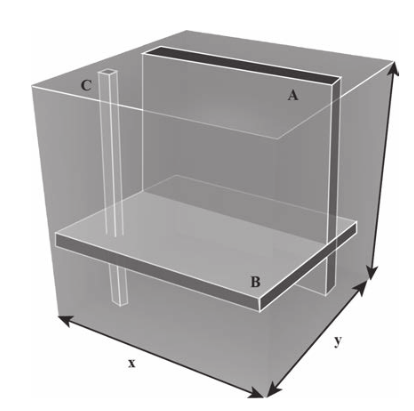
\includegraphics[width=10cm]{datacube.png}
%% \end{figure}

%% \begin{figure}[h]
%%   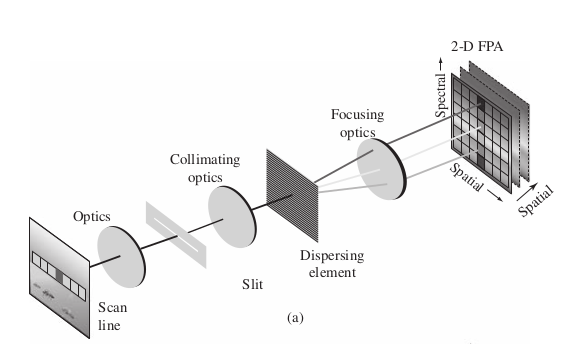
\includegraphics[width=10cm]{pushbroom.png}
%% \end{figure}


%% Different types of rigs:
%% \begin{itemize}
%%   \item Pushbroom scanner (ours)
%%   \item Staring System
%%   \item Fourier Transform Imaging Spectrometer (FTIS)
%% \end{itemize}


%% \subsection{Spatial Sampling}
%% \begin{itemize}
%%   \item ground resolution elements are mapped to picture elements (pixels)
%%   \item IFOV: Instantaneous Field of View
%%   \item Cross track dimension: the projection of the long axis of the slit (i.e. the axis of the pushbroom sensors)
%%   \item Along track dimension: the direction accumulated by traveling
%%   \item Ground Sample Distance: physical size of projected pixel element
%% \end{itemize}


%% \begin{figure}[h]
%%   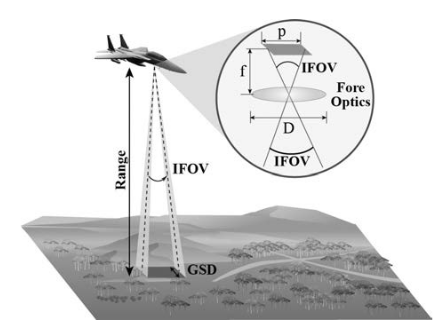
\includegraphics[width=10cm]{scanningProcedure.png}
%% \end{figure}


%% \subsection{Spectral Sampling}
%% \begin{itemize}
%%   \item Recovery of spectral info is imperfect due to finite sampling
%%   \item Spectral Response Function: is the weighing function that describes the wavelengths that are transmitted to a particular spectral sample
%% \end{itemize}

%% \subsection{Radiometric Sampling}
%% \begin{itemize}
%%   \item detector transforms  radiant power to electrical signal
%%   \item electrical signal converted to number via analog-to-digital converter
%%   \item photon detectors
%% \end{itemize}

%% \subsection{Signal Considerations}
%% Strength of signal is determined by:
%% \begin{itemize}
%%   \item Terrain composition affects amount of radiant energy reflected/emitted from ground resolution element
%%   \item Range: Intensity drops off by inverse square law. Further you are away, the worse the signal
%%   \item Spectral Bandwidth: output signal of detector element is proportional to spectral bandwidth of the detector
%%   \item Instantaneous Field of View: Decreasing IFOV increases spatial resolution but weakens the signal
%%   \item Dwell Time: the time required to sweep the IFOV across the ground resolution element, i.e. the time-on-pixel. Longer dwell time $\to$ more accumulated photons $\to$ more signal.
%% \end{itemize}





%% % -------------------------------------------------------------------- %

%% \section{Remote Sensing}

%% mention different types of satellite data platforms (mostly optical), differences in orbits, coverage, etc... Also good to discuss the increasing use of drones for a variety of applications including intelligent agriculture, geophysics, mapping, etc...



%% \subsection{Infrared Sensing Phenomenology}

%% Main passive sources of EM radiation for remote sensing are light emitted by the sun and the self-emission via black-body radiation of objects due to their temperature.

%% \subsection{Sources of Infrared Radiation}
%% \begin{itemize}
%% \item \textbf{spectral radiant exitance} power per unit area emitted by the sun. We can treat this as a black body with temperature $5800 K$, maximum emittance at $\lambda = 0.50$ $\mu m$.
%% \item The Earth is ~$300 K$ with maximum spectral radiant emittance at $\lambda = 9.7$ $\mu m$. This is known as the \textbf{thermal infrared}
%% \end{itemize}

%% \subsection{Atmospheric Propagation}

%% \begin{itemize}
%% \item Key parameter is the \textbf{path length} of atmosphered traveled through before it arrives at the remote sensing system. Main effects are:
%%   \begin{itemize}
%%   \item \textbf{Atmospheric Scattering}: diffusion of radiation by particles in the atmosphere
%%   \item \textbf{Absorption}
%%   \end{itemize}
%% \item Useful remote sensing spectral regions are obtained via the \textbf{Transmission Spectrum}.
%%   \begin{itemize}
%%   \item \textbf{Reflective Range}: $0.35-2.5$ $\mu m$. Dominated by solar illumination
%%   \item \textbf{Water Absorption}: $0.2-2.5$ $\mu m$.
%%   \end{itemize}
%% \item \textbf{Atmospheric Windows}: Regions of low atmospheric absorption
%% \end{itemize}

%% \subsection{Reflectance and Emissivity Spectra}

%% There are three processes that occur when EM radiation meets and interface:
%% \begin{enumerate}
%%   \item \textbf{Reflection}: Solar illumination dominates here. Consequently, this part of the spectrum is used to characterize the surface
%%     \begin{itemize}
%%     \item \textbf{Specular Reflectors}: Flat surfaces that act like mirrors, i.e. $\theta_i = \theta_r$.
%%     \item \textbf{Diffuse (Lambertian) Reflectors}: Rough surfaces that reflect uniformly in all directions.
%%     \item \textbf{Real Reflectors}: Somewhere between the specular and diffuse.
%%    \end{itemize}
%% \item \textbf{Absorption}
%% \item \textbf{Transmission}
%% \end{enumerate}

%% \begin{itemize}
%% \item Fractions vary as a function of $\lambda$
%% \item Remote sensing usually cares about \textit{diffuse} reflectors because this is the dominant type of most materials (water being an exception).
%% \item Reflectance of a material is characterized by its \textbf{Reflectance Spectrum}, that is, the percent of incident light reflected as a function of wavelength.
%%   \begin{itemize}
%%   \item Dips in reflectance spectrum are called \textbf{absorption features}
%%   \item Peaks are called \textbf{Reflectance Peaks}
%%   \end{itemize}
%% \item \textbf{Emissivity Spectrum}: The ratio of radiant emittance at a given temperature to the radiant emittance of a black body at the same temperature.
%% \end{itemize}




% -------------------------------------------------------------------- %

\section{Coordinated Robotic Teams}

we can discuss remote sensing, hyperspectral imaging, and the robot team here... Let's fetch some text from the 2019 paper.

\begin{itemize}
\item Remote Sensing: data acquisition, processing, and interpretation of images, and related data, obtained from aircraft and satellites that record the interaction between matter and electromagnetic radiation
\item Source: the source of electromagnetic radiation, e.g. the sun, black-body radiation, microwave radar, etc...
\item Atmospheric Radiation: The EM radiation propagating through the atmosphere. Moderated by various processes including absorption and scattering
\item Earth's Surface Interactions: Amount and spectral distribution of radiation emitted/reflected by the earth's surface. This depends on
  \begin{itemize}
  \item physical properties of the matter
  \item wavelength of EM radiation that is sensed
  \end{itemize}
\end{itemize}



%% % -------------------------------------------------------------------- %

%% \section{In-situ Chemical Sensing in Water}
%% Here we can give an overview of the sensors utilized on the boat for the robot team studies... We should include any information about the uncertainties. We can also comment on their use in fresh v.s. salt water environments, e.g. we should discuss fluorometers, sonar, and any other relevant sensors from the boat



% -------------------------------------------------------------------- %
\section{A Low Cost Sensor Network For Air Quality Monitoring}
The outdoor part here is optional. Here I seek to provide specific details of the classes of low cost sensors used for PM (optical particle counters based on Mie scattering), thermistors (for tempature), humidity sensors, pressure sensors, gas sensors, etc... This can be a rough outline for those that specifically are used in my research projects.



% -------------------------------------------------------------------- %
\section{PCO and The HEART Chamber}



Photocatalytic Oxidation (PCO) technology aims to reproduce the outdoor process of photolysis indoors, yielding oxidative molecules that can effectively reduce viruses, bacteria, fungi, and other contaminants, including VOCs. While the technology’s benefits have been well documented and replicated numerous times in real-world settings, we will focus attention, as directed by the RFI, on a highly rigorous approach to comprehensive measurements of indoor air quality and the resulting impacts that a technology, like Advanced Photocatalysis would have on any indoor atmosphere.

\begin{figure}[h]
  \centering
  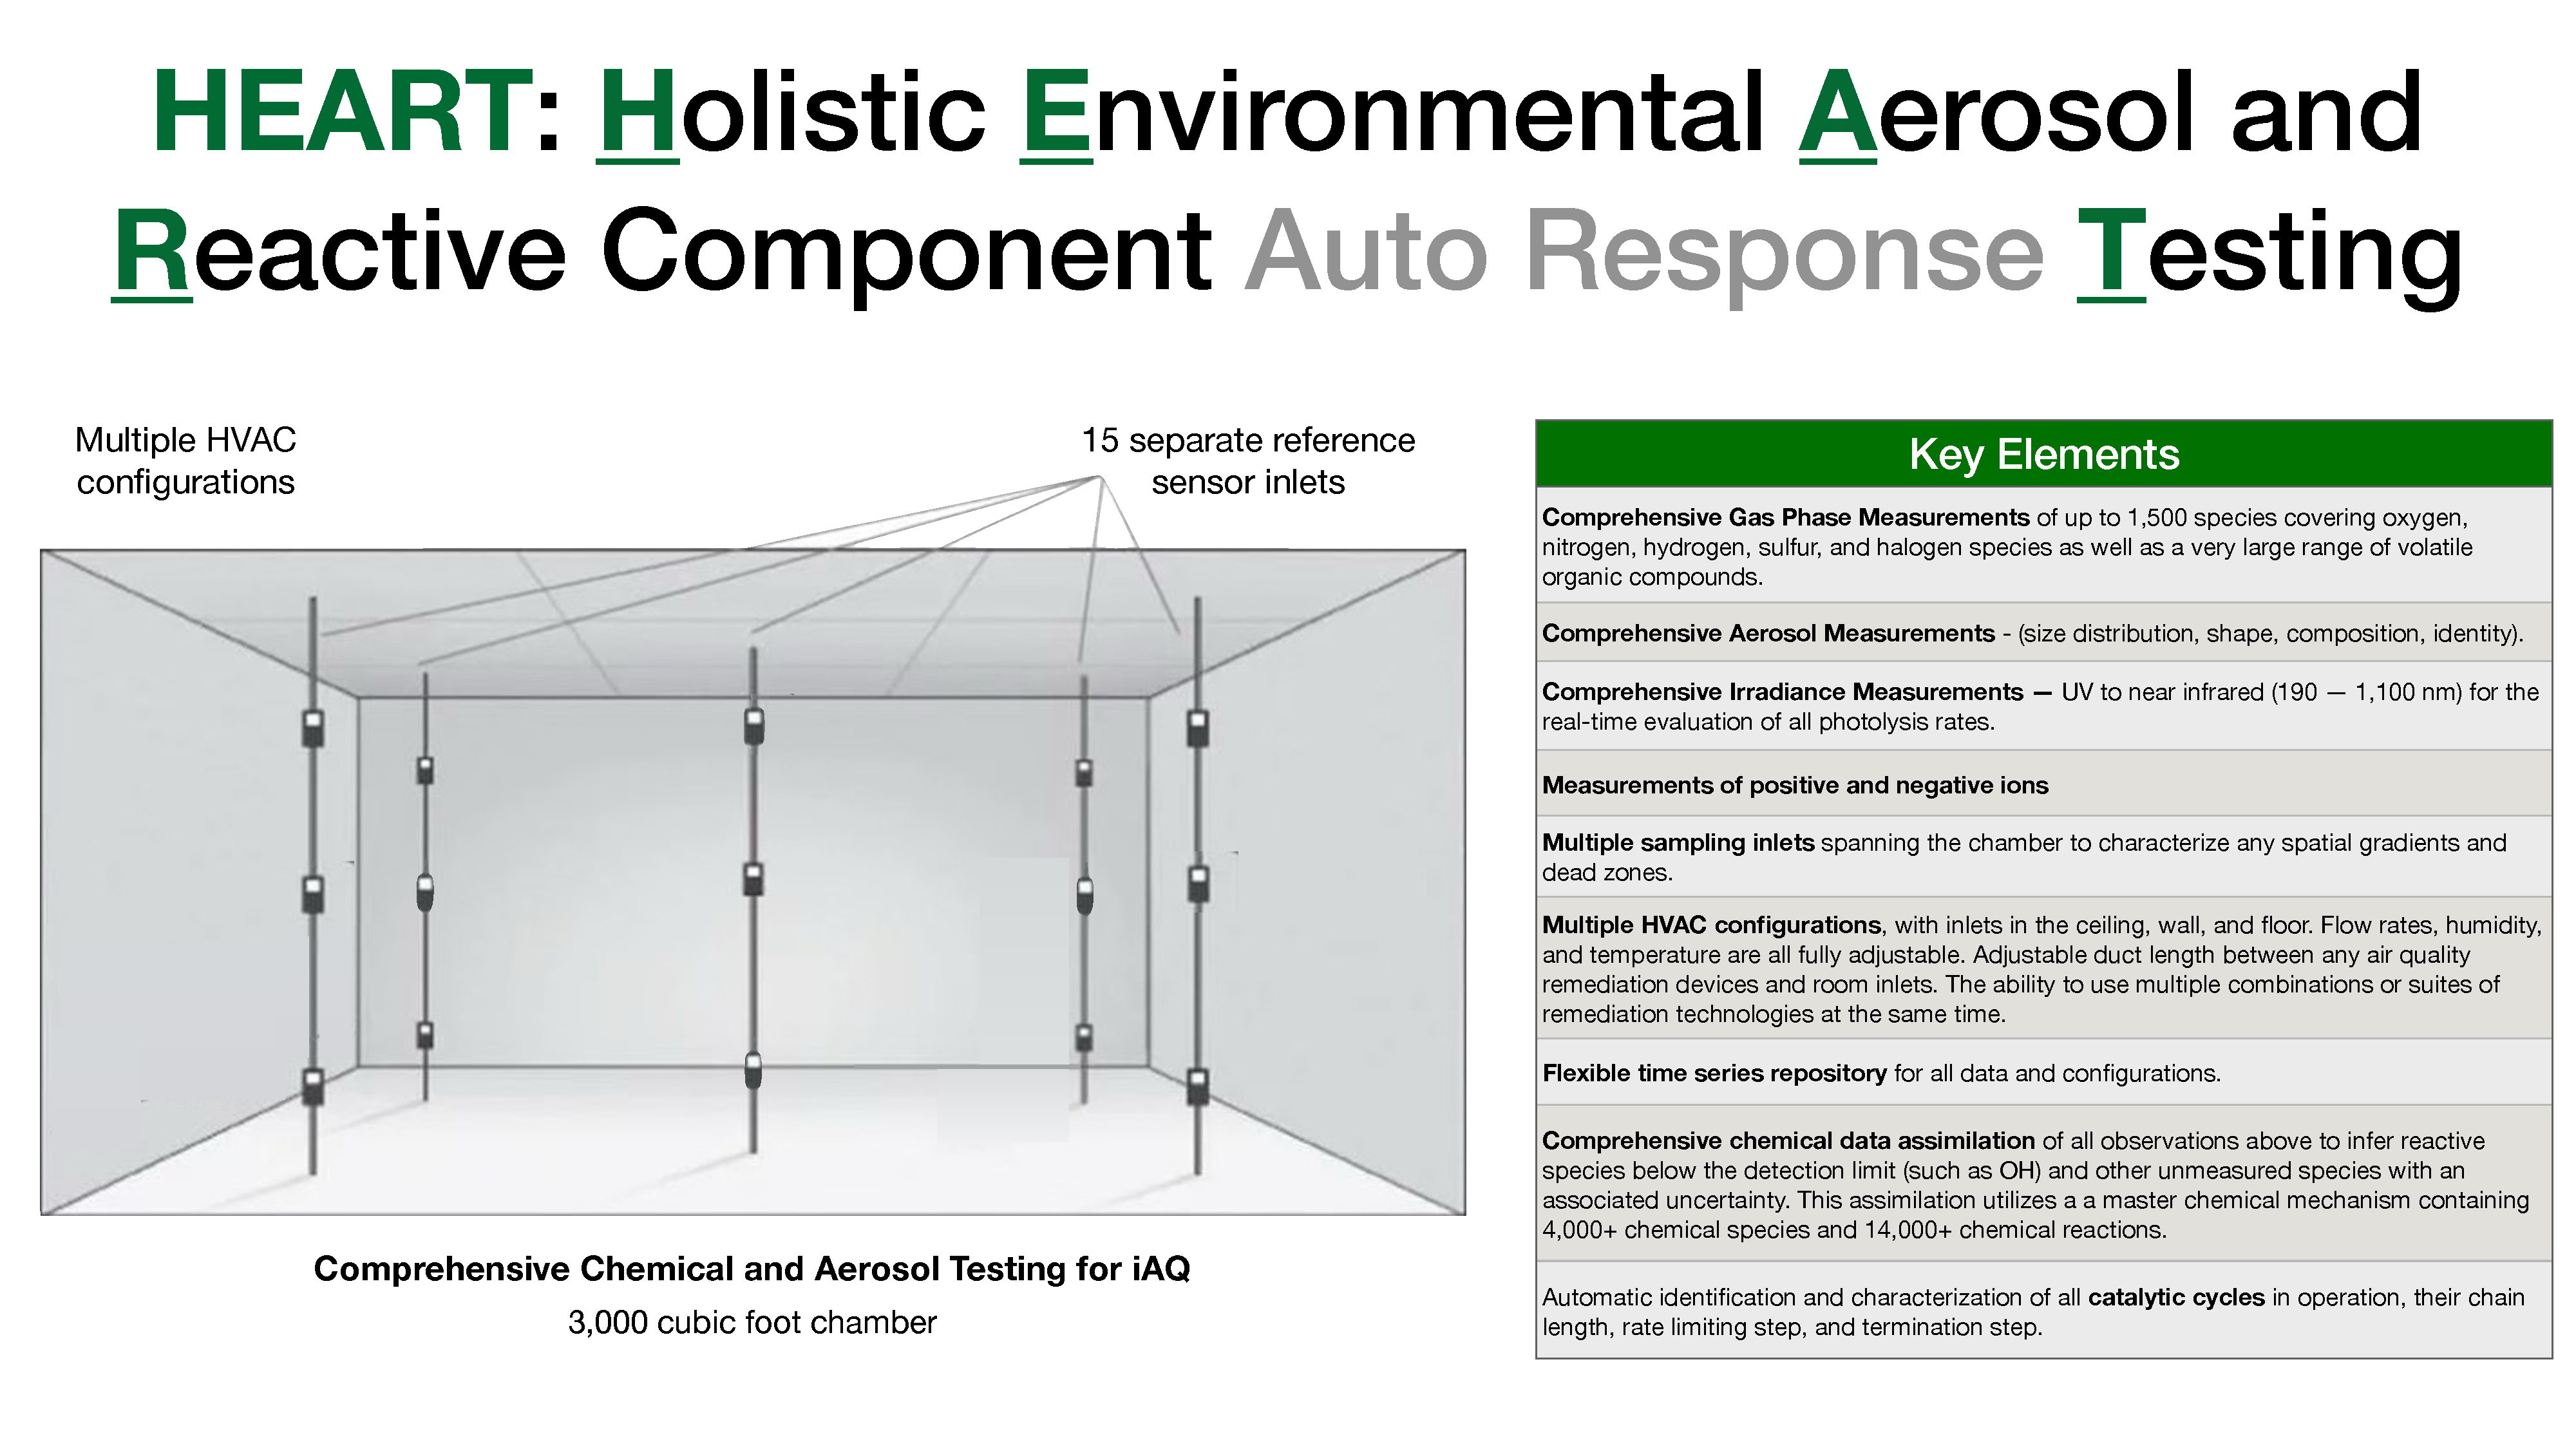
\includegraphics[width=\textwidth]{introduction/HEART-Details.pdf}
	\caption{Details of comprehensive chemical and aerosol testing for IAQ using HEART: Holistic Environmental Aerosol and Reactive Component Auto Response Testing.}
	\label{Figure.HEART-Details}
\end{figure}

The HEART test chamber is designed for comprehensive characterization of air quality including the chemical composition (characterizing hundreds of chemicals), positive and negative ion density, aerosol size (from 5 nm to 100 microns), detailed morphology (shape), and composition, and individual bio-aerosol particle recognition, along with the accurately characterized illumination environment characterized in more than 4,000 wavelengths from the UV to the near-infrared (190 — 1,100 nm) using a NIST calibrated spectrometer. The lighting environment is important, as, after all, air quality is atmospheric photochemistry in the indoor built environment, and photolysis is a key driver. Furthermore, some of the frequently advocated families of technologies make use of various parts of the ultraviolet spectrum. This high-energy region of the spectrum has important implications for indoor air quality.

\begin{figure}[h]
  \centering
  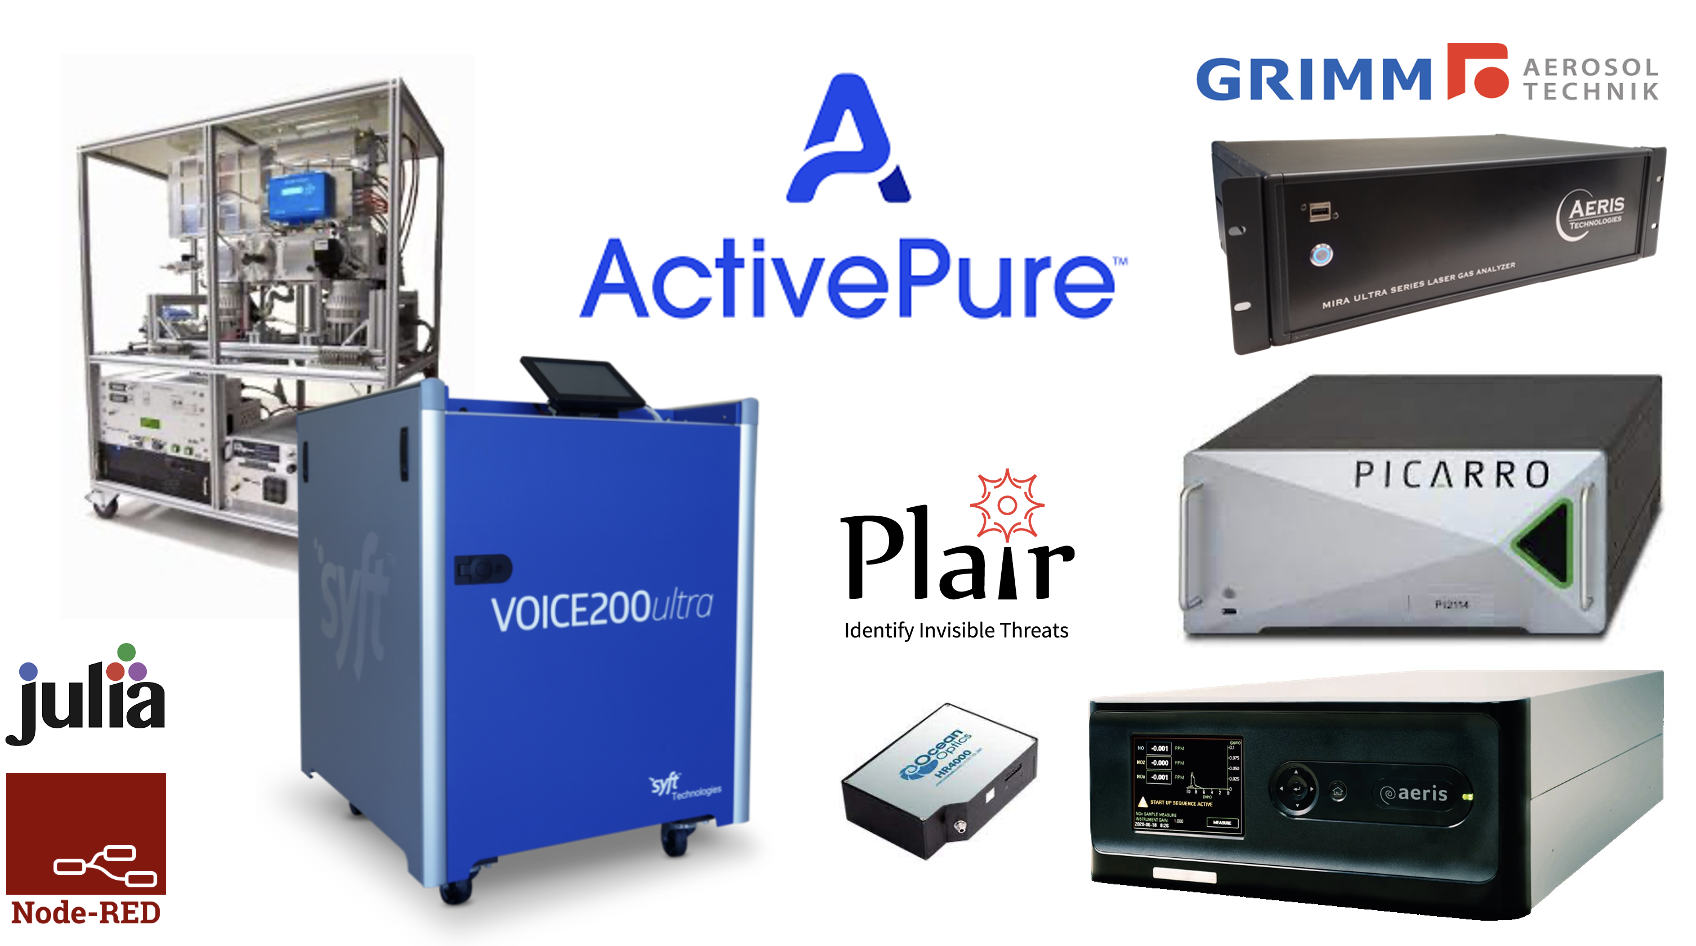
\includegraphics[width=\textwidth]{introduction/LabOverview.png}
	\caption{Visual overview of the various infrastructure components of the ActivePure lab. Note that the lab uses multiple instruments of those shown to accommodate the stated range of analytes.}
	\label{Figure.InstrumentOverview}
\end{figure}


This testing capability can be used in two modalities. The first is in a static test chamber with the same volume (3,000 cubic feet) as the EPA test chamber. The chamber is equipped with a comprehensive suite of sensors just described, holistically characterizing hundreds of chemicals, the size of individual aerosols from 5 nm to 100 microns, their morphology, and their composition. This is critical because remediation technologies, such as UV lights or various oxidation-based cleaners, may have a direct impact on the air's composition. Being able to comprehensively measure the gas phase oxygenated volatile organic compounds (OVOCs) and aerosol chemical composition is critical. Further, various cleaning compounds are often used in the indoor environment, introducing the possibility of significant levels of halogens. So as well as a suite of individual reference grade analyzers there is also a Syft 8 reagent ion mass spectrometer with a standard library of over 1,000 chemicals. The usual configuration used for the Syft is a large number of repeated sequential scans, each scan measuring a different family of species covering the nitrogen, hydrogen, sulfur, chlorine, bromine, and iodine families as well as the large range of volatile organic compounds. So for each measurement cycle, hundreds of species are measured. This is complemented by four  aerosol instruments characterizing the aerosol/bio-aerosol size distribution between 5 nm and 100 $\mu$m, the aerosol/bio-aerosol morphology, composition (using an aerosol mass spectrometer), and identity (with real-time machine learning providing a thousand member fingerprint for each individual particle,  so that once trained it can recognize on the fly every single aerosol/bio-aerosol and identify what mold, pollen, pathogen, etc that it is).

Further, it is inevitable that some chemical species, for example, reactive components such as OH, will typically be below the detection limit of the measurement systems. Information on these unmeasured reactive components is naturally embedded in the shape of the time-series observations of the chemical species they are reacting with and in the partitioning between the large number of measured components that they are reacting with. This information can be effectively extracted, together with associated uncertainty, using chemical data assimilation \cite{ISI:A1995TA29300008, Lary1999a, Lary2003a}, a technique we pioneered at the University of Cambridge and NASA, and now used routinely by the EPA, NASA and NOAA in providing air quality analyses and forecasts.

Hundreds of chemicals measured in real-time in the HEART chamber, along with high-resolution irradiance spectra used to calculate real-time photolysis rates and real-time aerosol measurements, are assimilated in a full chemical data assimilation system with a master chemical mechanism containing 4,000+ chemical species and 14,000+ chemical reactions. This enables us to accurately infer the abundance of unmeasured species, such as OH, with associated uncertainty. We use both 4D-Var chemical assimilation to initialize our system, followed by a full Kalman filter to time evolve the error covariance matrix. The chemical simulation and assimilation system won six NASA technology awards. This is the premier global approach for studying indoor air quality. Given the magnitude of the societal impacts of indoor air quality and preparing for any future pandemics, it is appropriate that the EPA uses a best-in-class methodology.

Furthermore, multiple HVAC configurations can readily be set up, with inlets located in the floor, ceiling, and walls. Further, the flow rates, humidity, and temperature can easily be adjusted, as can the length of the ductwork between any air quality remediation devices and the room inlets. In addition, various combinations or suites of remediation technologies can be used together.

In built-environment spaces, dead zones are a common issue. Fifteen inlets are strategically placed throughout the chamber to characterize the variability. The inlets are distributed across five vertical transects, with inlets at three vertical locations on each transect, 18 inches above the floor, on the centerline, and 18 inches below the ceiling.

The second modality for the test chamber is a mobile lab. This allows the performance of various remediation technologies to be tested in a wide range of ambient conditions. It also allows for the comprehensive exploration of the remediation technologies' effectiveness in a wide range of environments, from highly polluted such as in the Houston shipping channel, or downwind of a major forest fire, near a large composting facility, too unpolluted rural environments.





